% paper/sections/13e3_closed_interface_volume_gate.tex
%
% V12: closed-interface volume acceptance boundary for Chapter 14.2
% ═══════════════════════════════════════════════════════════════════════════════
\subsection{V12：閉界面体積の採用境界}
\label{sec:closed_interface_volume_gate}

\paragraph{目的．}
V12 は第~\ref{sec:val_oscillating_droplet}節の N=32 振動液滴を，
第13章側から監査する採用境界である．
このゲートは，閉界面振動液滴を新しい合格ベンチマークとして追加するものではない．
§14.2 の現行設定は \texttt{active\_geometry\_capillary} と
\texttt{compatibility\_projection} を用いる一方，本文には過去の
\texttt{sharp\_phase\_volume} / Ridge--Eikonal 経路の説明が残っていた．
したがって V12 では，現行設定が構築できること，
過去の sharp-volume 補修を現行状態空間に混入できないこと，
および現行設定の初期ステップ列が閉界面体積を受理できる段階に達していないことを
同じ実験スクリプトで固定する．

\paragraph{検査項目．}
入力は \texttt{experiment/ch14/config/ch14\_oscillating\_droplet.yaml} である．
V12 は三つの設定変種を作る：
(i) 現行 \texttt{active\_geometry\_capillary} +
\texttt{compatibility\_projection}，
(ii) そのまま \texttt{sharp\_phase\_volume} 制約だけを加えた負対照，
(iii) \texttt{ridge\_eikonal} +
\texttt{sharp\_phase\_volume} をアクティブ幾何の閉界面 endpoint に入れる負対照である．
さらに現行設定を短時間だけ進め，拡散質量
$M_\psi$ と P1 区分線形界面面積 $V_{\mathrm{P1}}$ を同時に読む．
この初期ステップ列は 1 周期受理ではなく，動的非一様格子の初期境界を測る診断である．

\begin{table}[htbp]
\caption{V12：閉界面体積の採用境界判定}
\label{tab:V12_closed_interface_volume_gate}
\centering
\PaperTableDenseSetup
\begin{tabularx}{\linewidth}{@{}>{\raggedright\arraybackslash}p{0.28\linewidth}>{\raggedright\arraybackslash}X>{\raggedright\arraybackslash}p{0.18\linewidth}@{}}
\toprule
項目 & 観測と解釈 & 判定 \\
\midrule
現行設定の構築 & \texttt{active\_geometry\_capillary} +
\texttt{compatibility\_projection} は構築可能であり，
再初期化の体積診断は既定の \texttt{diffuse\_mass} である． & \checkmark 境界 \\
sharp-volume 追加 & \texttt{compatibility\_projection} に
\texttt{sharp\_phase\_volume} を足す経路は
\texttt{ValueError}: volume constraint is only implemented for
\texttt{ridge\_eikonal} で停止する． & \checkmark 不合格停止 \\
Ridge--Eikonal 追加 & \texttt{active\_geometry\_capillary} の
\texttt{geometric\_cell\_fraction} endpoint は
\texttt{algorithm} を \texttt{none} または
\texttt{compatibility\_projection} に限定するため，
\texttt{ridge\_eikonal} は停止する． & \checkmark 不合格停止 \\
周期計量 & 現行格子の $\sum_C |C|$ と周期一意領域面積はいずれも
$4.000000000000\times10^{-4}$ であり，relative overcount は $0$． & \checkmark \\
現行設定の初期ステップ & 1 step では
$t=2.652412244614\times10^{-5}$,
$\Delta M_\psi/M_{\psi,0}=-1.080216\times10^{-1}$,
$\Delta V_{\mathrm{P1}}/V_{\mathrm{P1},0}=-5.993794\times10^{-3}$．
2 step 目は射影後の面履歴を格子再構築後の active reprojector が
再射影できず停止する． & \checkmark 診断 \\
1 周期標準実行 & §14.2 の既存 1 周期標準実行は有限値で完走したが，
拡散質量保存診断 $=3.5495\times10^{-1}$，
P1 区分線形界面面積ドリフト $+25.8919\%$ のため受理しない． & \checkmark 境界 \\
\bottomrule
\end{tabularx}
\end{table}

\begin{figure}[htbp]
\centering
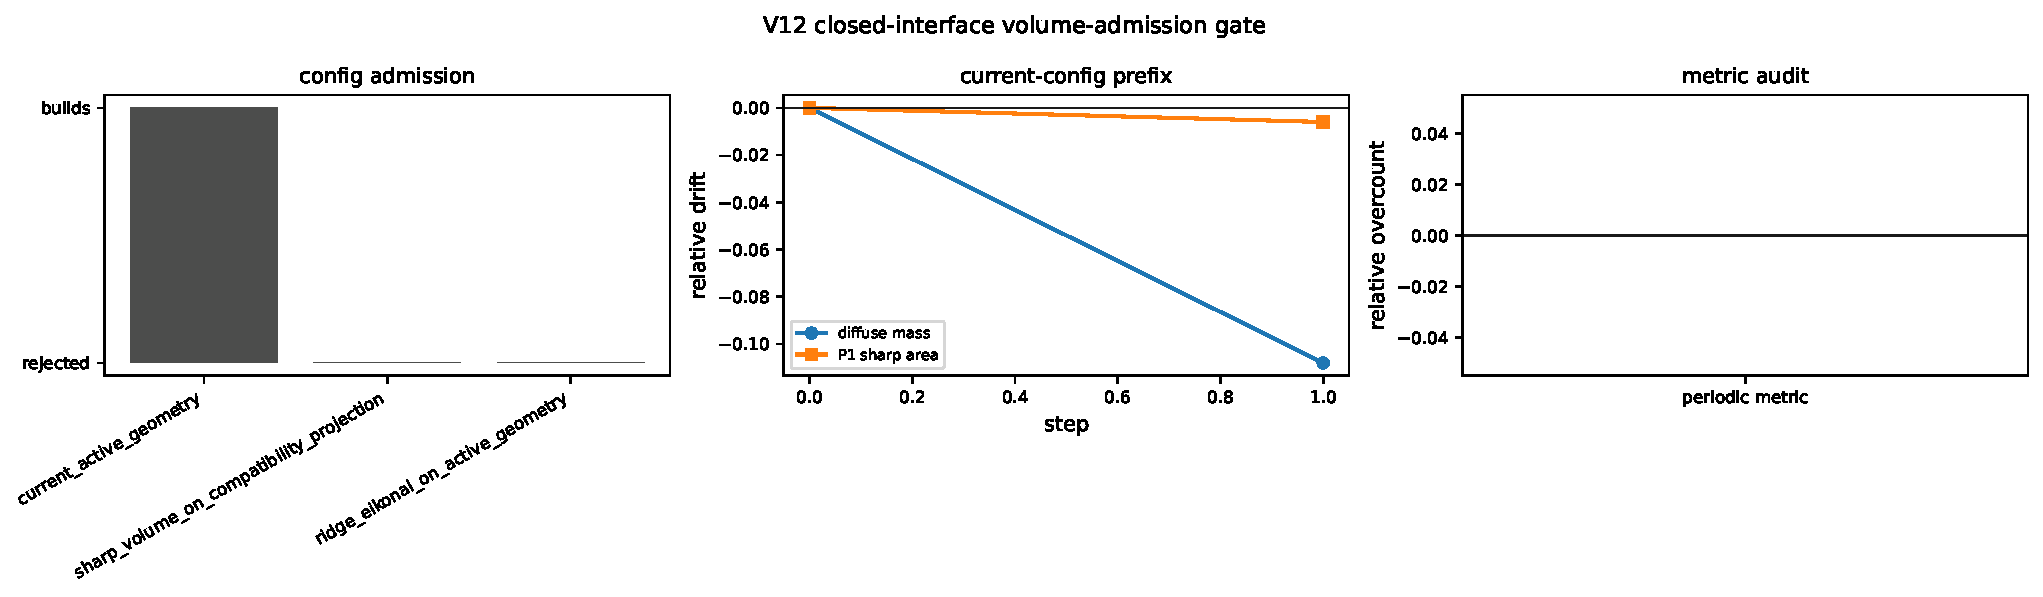
\includegraphics[width=0.96\linewidth]{figures/ch13_v12_closed_interface_volume_gate.pdf}
\caption{V12：閉界面体積の採用境界．
左は現行設定と二つの過去の補修候補の構築可否，
中央は現行設定の初期ステップにおける拡散質量および P1 区分線形界面面積ドリフト，
右は周期計量の重複監査を示す．}
\label{fig:V12_closed_interface_volume_gate}
\end{figure}

\paragraph{判定．}
V12 の結論は二つである．
第一に，§14.2 で \texttt{sharp\_phase\_volume} / Ridge--Eikonal を
現行標準設定として読む記述は陳腐化しており，削除または負対照へ移す必要がある．
第二に，閉界面の標準実行経路は
同一 P1 面積を輸送・格子再構築・再写像・プロファイル復元の全段で保持する経路を
まだ持たないため，1 周期振動液滴を合格ベンチマークへ昇格できない．
したがって V12 は，V1--V11 の再実験要求ではなく，
第~\ref{sec:val_oscillating_droplet}節の記述更新と今後の実装境界を決める
採用境界として扱う．
